\chapter{COLREGS Compliant System}
\label{chap:4_COLREGS_Compliant_Guidance_System}

    %%%%%%%%%%%%%%%%%%%%%%%%
    % Grammarly: 100/100
    %%%%%%%%%%%%%%%%%%%%%%%%
    Is this chapter, we present the architecture of the \ac{USV} system we developed, and describe in detail the main contribution of this work, our COLREGS-compliant local planner. 
    %In section \ref{sec:sys_arch} we show each component of the \ac{GNC} system and in section \ref{sec:local_planner} we detail the COLREGS-compliant behavior, Figure \ref{fig:local_planner_flow} summarize the whole flow.

\section{Assumptions and Limitations}
\label{sec:assum_and_limits}

%AMA evita secoes formatadas dessa forma. tem q ter pelo menos um frase introduzindo a secao. por exemplo: The following assumptions and limitations apply for this work:

    \begin{enumerate}
        
        %%%%%%%%%%%%%%%%%%%%%%%%
        % Grammarly: 100/100
        %%%%%%%%%%%%%%%%%%%%%%%%
        \item \ac{ROS} compatibility: the whole system we developed and present in this chapter is ROS compatible. We developed it following \ac{ROS} concepts and development paradigms. We avoided unnecessary implementation details in this chapter and focused on explaining the general operation of the system. %Implementation details are available in Appendix \ref{append:ros_implementation}.
        
        %%%%%%%%%%%%%%%%%%%%%%%%
        % Grammarly: 100/100
        %%%%%%%%%%%%%%%%%%%%%%%%
        \item Encountering between power-driven vessels: we developed our system to run on power-driven vessels and considered the encountering between vessels of the same type. Concerning COLREGS, the encounter between different types of vessels imposes different ways to avoid collisions. Our system, in its current state, may be able to avoid collision with other types of vessels, but the avoidance strategy will always consider the other vessel as a power-driven vessel.

        %%%%%%%%%%%%%%%%%%%%%%%%
        % Grammarly: 95/100
        %%%%%%%%%%%%%%%%%%%%%%%%
        \item Encountering with one vessel: currently, we developed our system to perform COLREGS-compliant collision avoidance with only one vessel at a time. In a multiple vessels encounter scenario, our system may be able to perform evasive actions but we do not have any assurance regarding COLREGS-compliance for this scenario.

    \end{enumerate}

\section{System Architecture}
\label{sec:sys_arch}

    %%%%%%%%%%%%%%%%%%%%%%%%
    % Grammarly: 100/100
    %%%%%%%%%%%%%%%%%%%%%%%%
    Our system consists of 3 main modules: guidance, navigation, and control. In a high-level view
    %AMA conception pode ser interpretado de outra forma. troquei por view
    , the navigation system is responsible for gathering information about the environment and the own vessel. The guidance system performs decision making, using information gathered by the navigation system, and then generates commands to the control system in order to achieve a goal location. The control system maps the commands received from the guidance system into actuation commands to change \ac{USV}'s state. In Figure \ref{fig:gnc_arch}, we present an overview of the system, and in next sections - \ref{sec:chap4_navigation} Navigation, \ref{sec:chap4_control} Control, and \ref{sec:chap4_guidance} Guidance, - we describe each module in detail.

    %%%%%%%%%%%%%%%%%%%%%%%%
    % Grammarly: 100/100
    %%%%%%%%%%%%%%%%%%%%%%%%
    Beyond the \ac{GNC} components of our system, we show in Figure \ref{fig:gnc_arch}, the mission planner, and gazebo modules. The mission planner module generates goals to be followed by the \ac{USV}. The mission planner is an independent ROS-package; we developed it as an external module. Thus it can be replaced by any other module compliant to the standard move\_base ROS goal publishing\footnote{Read more about it in http://wiki.ros.org/move\_base}. The gazebo module is a USV\_sim module to interacting with the objects of the simulation; through it, we can change and gather the \ac{USV}'s state and the environment state.

    \begin{figure}
        \centering
        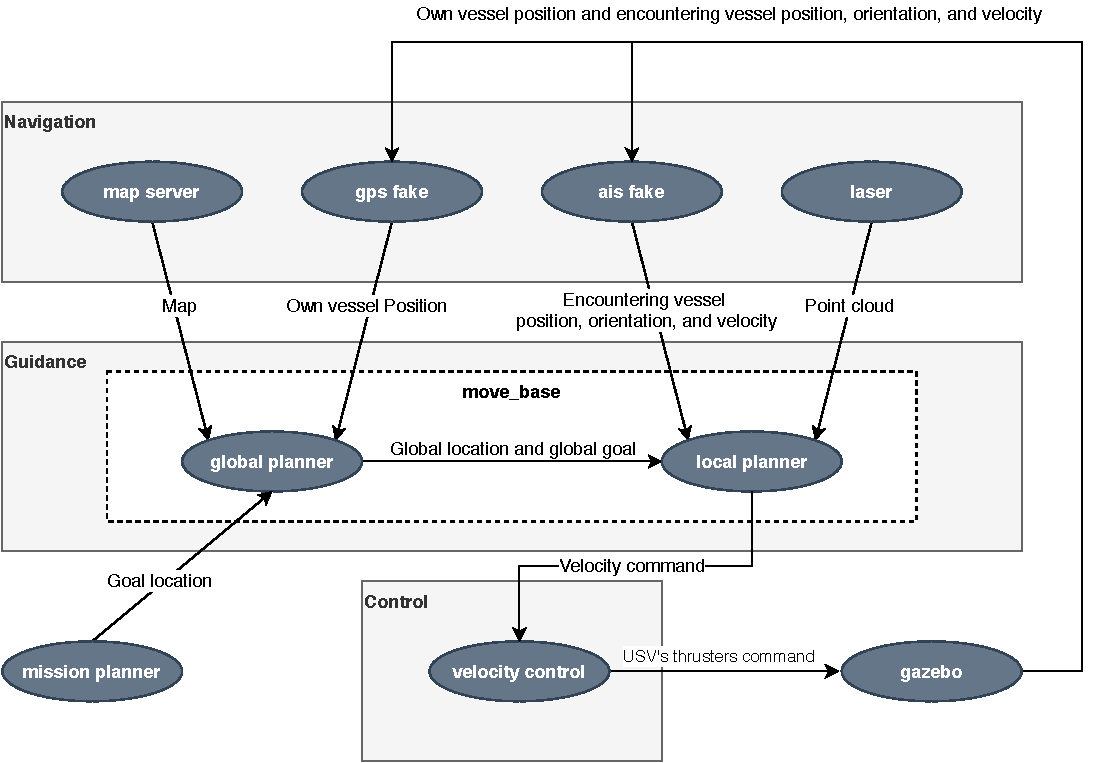
\includegraphics[scale=0.9]{figs/Chap4/gnc_arch.pdf}
        %%%%%%%%%%%%%%%%%%%%%%%%
        % Grammarly: ?/100
        %%%%%%%%%%%%%%%%%%%%%%%%
        \caption{Guidance, Navigation, and Control Architecture of our System. In this Figure, we can observe the composition of the system, the messages exchanged between modules, and our contributions.}
        \label{fig:gnc_arch}
    \end{figure}
    
        \subsection{Navigation}
    \label{sec:chap4_navigation}
    The navigation system gathers data for environment perception and state estimation. The navigation system consists of the following sub-modules:
    
    \begin{itemize}
    
        %%%%%%%%%%%%%%%%%%%%%%%%
        % Grammarly: 99/100
        %%%%%%%%%%%%%%%%%%%%%%%%
        \item \textbf{map server}: the map server module is responsible for making the global map available for the guidance system. The map is generated before the start of the \ac{USV} mission. Both the map and an adapted version of the map server module were made available by the USV\_sim maintainers.
    
        %%%%%%%%%%%%%%%%%%%%%%%%
        % Grammarly: 99/100
        %%%%%%%%%%%%%%%%%%%%%%%%
        \item \textbf{gps fake}: the gps fake module is a simplification of a real GPS; its information is extracted directly from the simulator; that is, it does not perform a simulated query to satellites. The gps fake module performs a simple query to the gazebo module in order to acquire a 3-tuple - (x, y, z) - for determination of the position of the \ac{USV} in the global reference frame. This module can be replaced by another localization method, such as \ac{AMCL}\footnote{http://wiki.ros.org/amcl} or a real GPS device. We integrated this module into the system as a contribution to this work.\footnote{Implementation based on http://wiki.ros.org/fake\_localization}
    
        %%%%%%%%%%%%%%%%%%%%%%%%
        % Grammarly: 99/100
        %%%%%%%%%%%%%%%%%%%%%%%%
        \item \textbf{ais fake}: the ais fake module is a simplification of the real AIS system\footnote{A real AIS module must respect NMEA legislation, refer to NMEA for specification: https://www.nmea.org/Assets/nmea\%20collision\%20avoidance\%20through\%20ais.pdf} which is used on vessels sailing on the high seas. The ais fake module provides the position and velocity of another vessel. The ais fake generates its information from a direct query to the simulator data. We developed and integrated this module into the system as a contribution to this work.
    
        %%%%%%%%%%%%%%%%%%%%%%%%
        % Grammarly: 100/100
        %%%%%%%%%%%%%%%%%%%%%%%%
        \item \textbf{laser}: this module provides the location of bodies of mass that reflect the laser light beam through an ordered 3-tuple - (x, y, z) position referring to the global frame. In our system, the laser module performs detection of static and dynamic obstacles, and every detection generates an update on the local cost map. This module is available as a standard module in USV\_sim. We configured this module to be compatible with the following requirements: laser beam range up to 25m and 360º detection capability; both specifications are compatible with real lasers, for example, the Slamtec RPLIDAR A3 laser \cite{RPLidarA3}.
    
    \end{itemize}
    
    % \subsection{Guidance}
    % O sistema de guidance é composto pelos seguintes submódulos:
    % \begin{itemize}
    %     \item \textbf{global\_planner}: O módulo global\_planner é responsável por .
    %     \item \textbf{local\_planner}: .
    % \end{itemize}
    
    \subsection{Control}
    \label{sec:chap4_control}
    
        %%%%%%%%%%%%%%%%%%%%%%%%
        % Grammarly: 100/100
        %%%%%%%%%%%%%%%%%%%%%%%%
        The control system is composed of the velocity controller module. The velocity controller module maps velocity commands received from the local planner into actuation commands. Then the velocity controller module interacts directly with the simulator and sends actuation commands to modify the \ac{USV}'s state.  This module is available as a standard module in USV\_sim, and we used it without any modifications.
        
    \subsection{Guidance}
    \label{sec:chap4_guidance}

        %%%%%%%%%%%%%%%%%%%%%%%%
        % Grammarly: 100/100
        %%%%%%%%%%%%%%%%%%%%%%%%
        As shown in Figure \ref{fig:gnc_arch}, the guidance module is mainly composed of global and local planners. We implemented both planners inside the ROS move\_base environment. For global planning, we use move\_base standard A* search\footnote{http://wiki.ros.org/global\_planner?distro=kinetic}, and for local planning, we developed our own COLREGS-compliant A*. The global planner determines the global route, and the local planner is always responsible for generating velocity commands to move the \ac{USV}, regardless of whether there are obstacles nearby or not. The moves\_base ROS structure imposes this style.
        
        %%%%%%%%%%%%%%%%%%%%%%%%
        % Grammarly: ?/100
        %%%%%%%%%%%%%%%%%%%%%%%%
        Beyond planners, the guidance module has cost maps. Cost maps are data structures composed of cells to store information about each position of the environment (see Figure \ref{fig:costmaps}). There is a cost map for each planner, and each cell of a cost map has a cost value (range from 0 to 255, where a cost greater than 250 represents an obstacle). Thus, planners can search for optimized paths. 
        
        Our local cost map is a 100x100 grid, representing a 20mx20m area with 1:0.2 resolution, resulting in a search space of 10000 cells. The local cost has the vessel around its center with some variation of at most 2 grid cells due to approximation error when converting global position to local position.
        
        \begin{figure}[H]
            \centering
            % 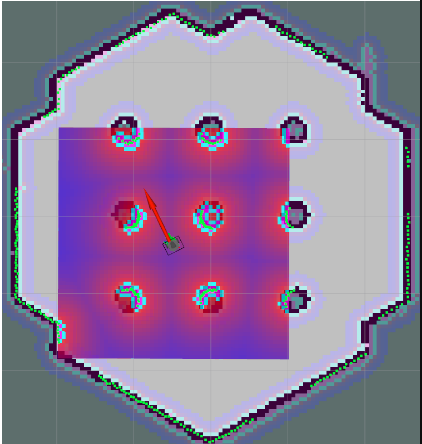
\includegraphics[scale=1.0]{figs/Chap4/costmaps_ros2.png}
            %Figure extracted from ROBOTIS emanual (http://emanual.robotis.com/docs/en/platform/turtlebot3/ros2\_navigation2/)
            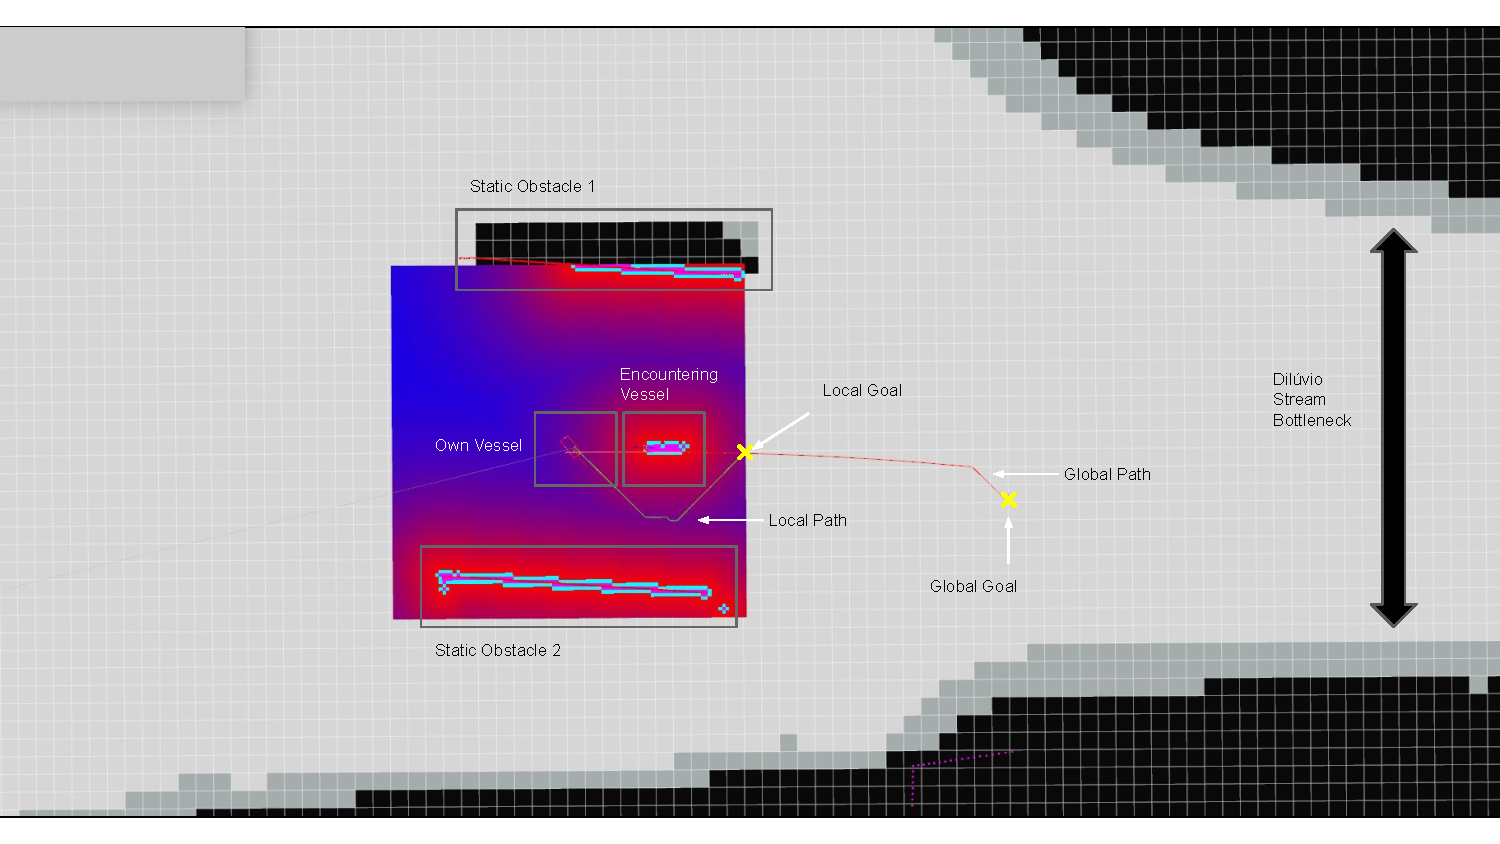
\includegraphics[scale=0.67]{figs/Chap4/costmaps.pdf}
            %%%%%%%%%%%%%%%%%%%%%%%%
            % Grammarly: 100/100
            %%%%%%%%%%%%%%%%%%%%%%%%
            \caption{In this Figure we show a practical exemplification of global and local cost maps. In the center of the Figure, we have a robot capable of detecting obstacles in its proximity using a laser.  Every red dot represents a laser contact in obstacles surface. Around the robot position, we can see a squared grid with a gradient from blue to red, indicating proximity to obstacles, this squared grid is a local cost map. All information out of the local cost map composes the global cost map. }
            \label{fig:costmaps}
        \end{figure}

        \subsubsection{Local Planner}
        \label{sec:local_planner}
        
            %%%%%%%%%%%%%%%%%%%%%%%%
            % Grammarly: 100/100
            %%%%%%%%%%%%%%%%%%%%%%%%
            The local planner module is responsible for the local path planning and the reactive behavior of our system. When encountering static or dynamic obstacles, 
            %AMA acho bo mincluir isso. o que acha ? within the local cost map area,
            the local planner reacts generating collision-free local paths, while keeping aligned with the global route generated by the global planner. For path finding, our local planner performs A* search in the local cost map. Performance evaluation is presented in the next chapter.\todo{Missing time complexity analysis? Missing general A* algorithm flow?}
            
            %%%%%%%%%%%%%%%%%%%%%%%%
            % Grammarly: 99/100
            %%%%%%%%%%%%%%%%%%%%%%%%
            Our local planner performs COLREGS-compliant path planning using a modified version of \ac{ATC} presented by Agrawal \etal~\cite{Agrawal2015COLREGS}. With \ac{ATC}, we restrict the search space, building virtual obstacles in no COLREGS-compliant locations, see Figure \ref{fig:atc}. The path planner creates virtual obstacles from the encountering vessel location until the local cost map border. Virtual obstacles increase the cost of cells to a value above the A* acceptance. Thus, when searching for routes to reach the goal position, A* is unable to choose regions that violates COLREGS.
            
            Virtual obstacles occupy an area $w \times m$ where $w$ is the width of our own vessel in the local frame (2 local cost map cells) and $m$ is the distance between the other vessel and the corresponding border. In general $m$ is around the half of of the grid side size (50 cells) once the local cost map usually has the vessel nearby its center. 
            %AMA adicionei usually e nearby p relativar esse comentario, q nao eh necessariamente verdade sempre. ainda assim, acho q 'has the vessel' esta um pouco confuso pois nao esta claro se eh OV ou o EV.
            
            \begin{figure}[H]
                \centering
                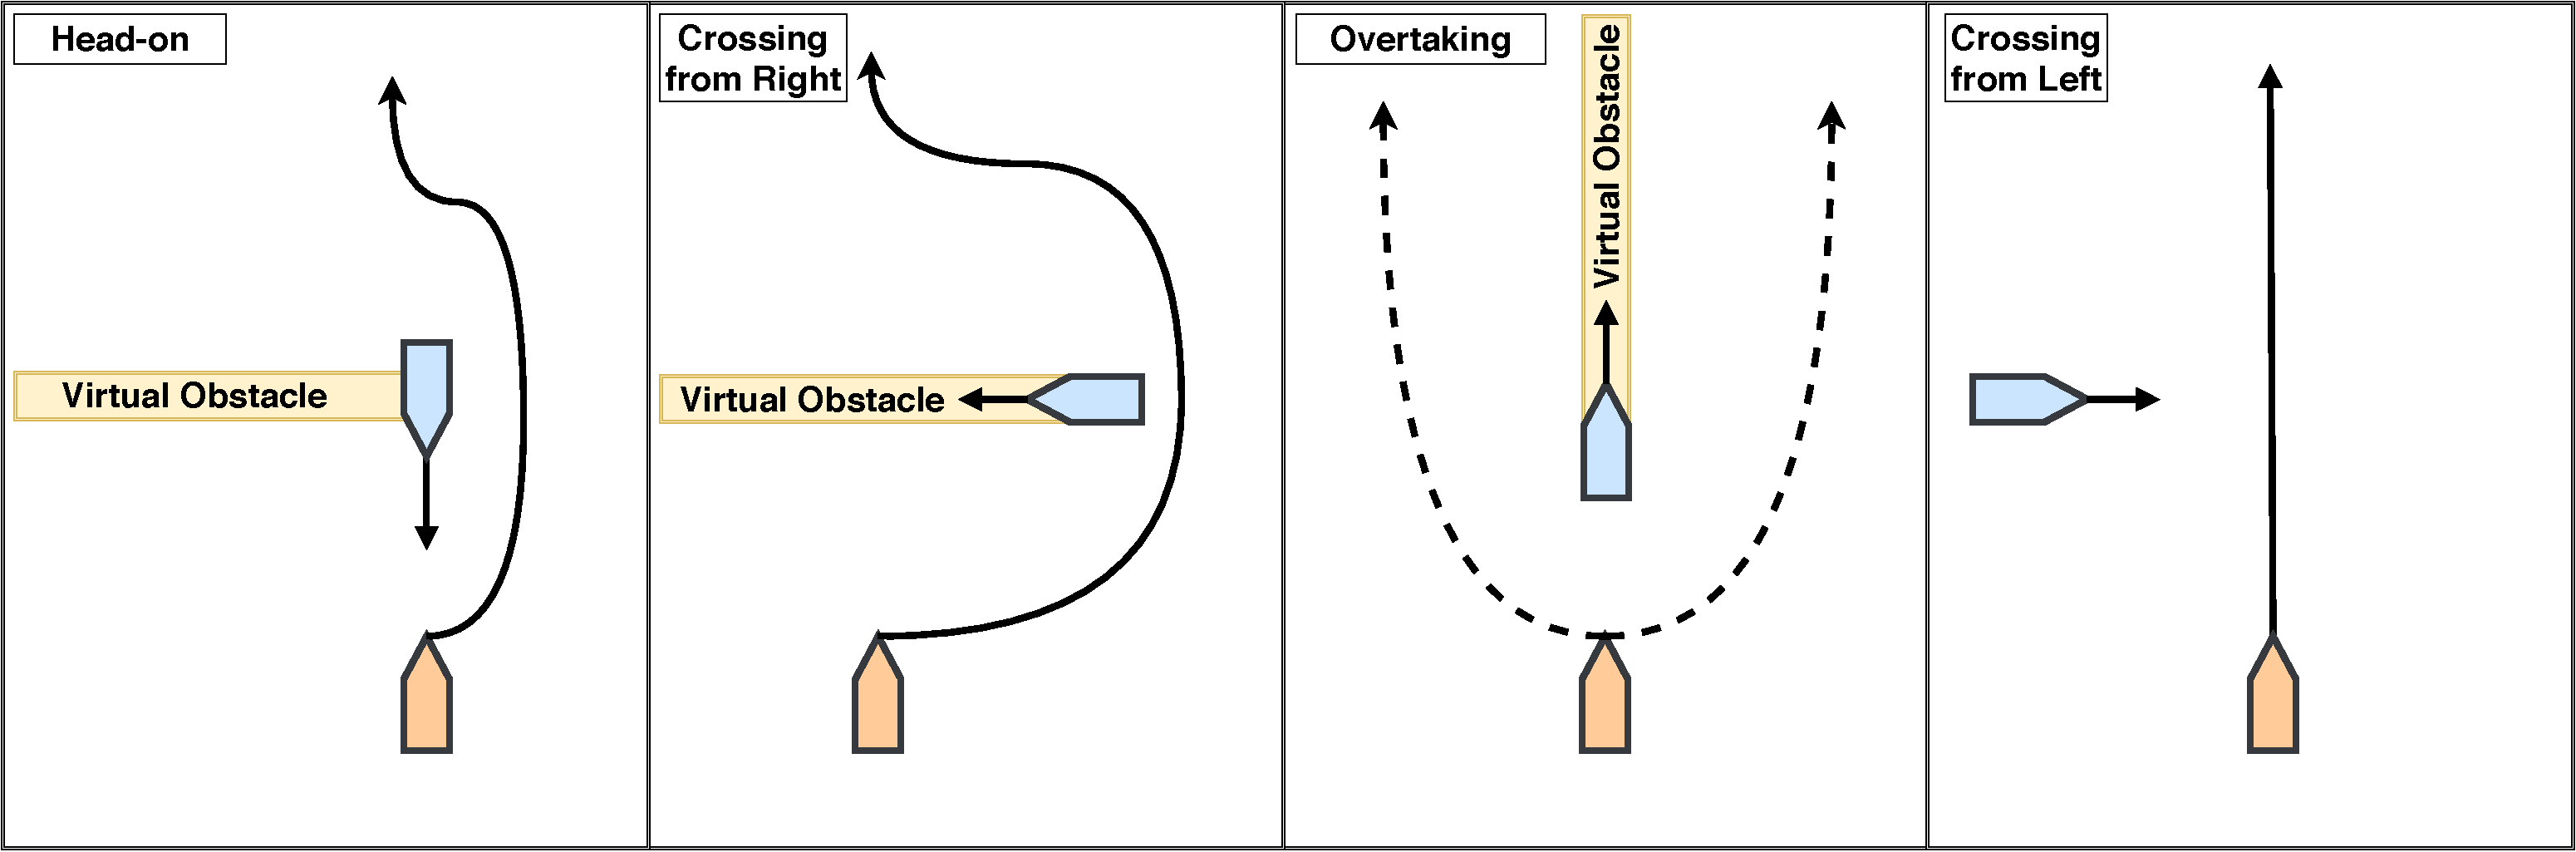
\includegraphics[scale=0.32]{figs/Chap4/atc.pdf}
                %%%%%%%%%%%%%%%%%%%%%%%%
                % Grammarly: 99/100
                %%%%%%%%%%%%%%%%%%%%%%%%
                \caption{\ac{ATC} for COLREGS Encounters: For head-on and crossing from right encounters, the local path planner creates the virtual obstacle in the portside side, forcing the planner to determine a route through the \ac{USV}'s starboard side, featuring COLREGS-compliant behavior. For overtaking, COLREGS specifies that the vessel performing overtaking should not generate another crossing encounter during its operation. Thus the local planner creates a virtual obstacle in the direction in front of the encountering vessel. For crossing from left, no virtual obstacle is created once COLREGS specifies that in this situation, the vessel coming from left is responsible by the avoidance, and the other vessel must stand-on its current course.
                %AMA informa na legenda q o barco azul eh o encountering
                }
                \label{fig:atc}
            \end{figure}

            %%%%%%%%%%%%%%%%%%%%%%%%
            % Grammarly: 99/100
            %%%%%%%%%%%%%%%%%%%%%%%%
            The local planner generates at every computation cycle a velocity command for the vessel, the command is composed of linear and angular velocities. The velocity command is sent to the control system and determines the local behavior of the \ac{USV}. The local planner generates the velocity command based on the path found after executing the \ac{ATC} A* search method. The local planner has an internal control system based on proportional controllers that generates the velocity command considering the next desired pose and the current pose of the \ac{USV}\footnote{We developed the controller based on http://wiki.ros.org/turtlesim/Tutorials/Go\%20to\%20Goal}. In Equation \ref{eq:cmd_vel}, we show linear and angular velocities composition. We empirically defined values for $K_{p_{l}}$, and $K_{p_{a}}$. Linear velocity is proportional to the distance between the goal and \ac{USV}'s current position. While angular velocity is proportional to the difference between the \ac{OV}'s current angle and the steering angle\footnote{http://street.umn.edu/VehControl/javahelp/HTML/Definition\_of\_Vehicle\_Heading\_and\_Steeing\_Angle.htm} related to the goal and \ac{OV}'s current position.
            
            \begin{equation}
            \label{eq:cmd_vel}
            \begin{split}
                Vl = K_{p_{l}}\ *\ G_{l} \\
                Va = K_{p_{a}}\ *\ G_{a}
            \end{split}
            \end{equation}
            \\
            where $Vl$ means linear velocity, $Va$ means angular velocity, $K_{p_{l}}$ = 0.075,$K_{p_{a}}$ = 0.75, 
            
            \[ G_{l} = \sqrt{(x_{g} - x_{c})^2- (y_{g} - y_{c})^2}\], and 
            \[G_{a} = atan2\footnote{https://en.wikipedia.org/wiki/Atan2}(x_{g} - x_{c}, y_{g} - y_{c}) - \theta_{c}\]
            \\
            where $g$ denotes goal position, and $c$ denotes \ac{USV}'s current pose, 
            
            \todo{add a paragraph describing how to create the Virtual Obstacle and determine its location related to the 3-tupla (x,y,ori)}
            
            In Figure \ref{fig:local_planner_flow} we summarize our planner's operating sequence. Based on the decisions we enumerated the following list: 
            
            \begin{enumerate}
            
                \item The proposed local planner waits to receive a mission. As discussed earlier, missions are locations goals generated by the mission planner module;
                
                \item After receiving a goal, the planner evaluates information received from the ais fake module. If is there a vessel near, the local planner identify the type of COLREGS encountering and then creates a virtual obstacle;
                
                \item The local planner validates if the local goal can be used as a goal for the A* method. A goal is considered not valid when an obstacle occupies the same location. When there is an obstacle occupying the same location as the local goal, the local planner searches for another possible local goal within the local cost map, through a reverse search into the global planner path. If the goal is valid, we run A*.
                
                The local goal is defined as being the farest location in the path defined by the global planner within the local cost map (see Figure \ref{fig:costmaps});
                
                \item After A*, a path may have been generated or not. If there is a path, the planner generates a velocity command;
                
                \item If the last execution of \ac{ATC} A* had a valid goal, the local planner uses the last velocity command. If there is no last valid goal, the local planner generates a stop command.

            \end{enumerate}
        
        \begin{figure}[H]
            \centering
            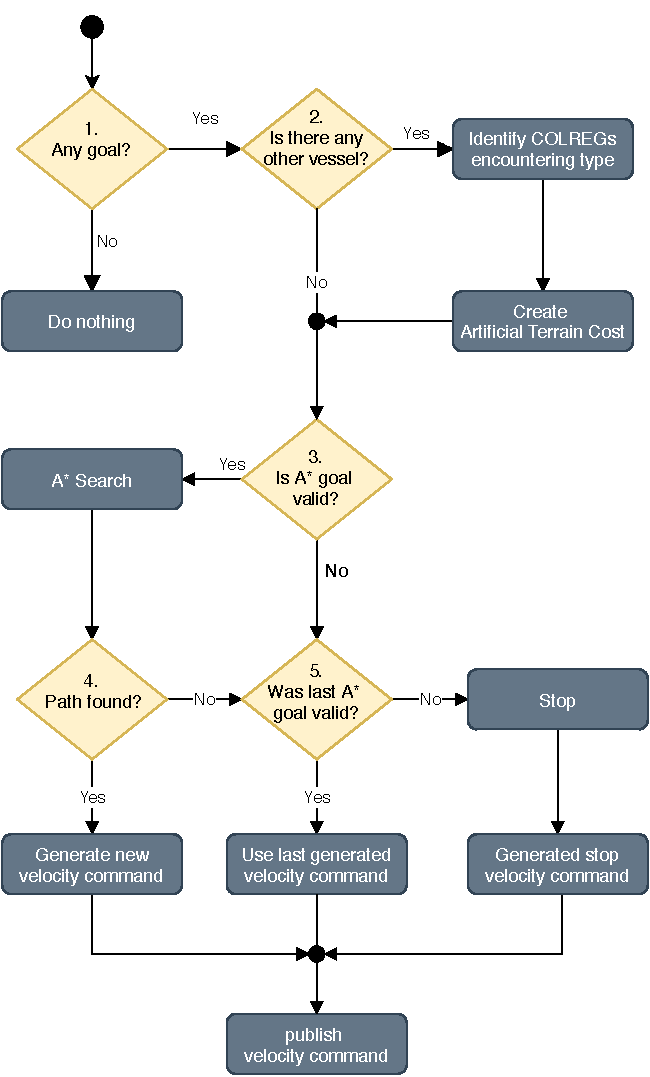
\includegraphics[scale=0.95]{figs/Chap4/local_planner_flow.pdf}
            %%%%%%%%%%%%%%%%%%%%%%%%
            % Grammarly: 100/100
            %%%%%%%%%%%%%%%%%%%%%%%%
            \caption{Here we present a simplification of the sequential execution of our COLREGS-compliant path planning method. Some details are omitted to facilitate general understanding on how the system works.}
            \label{fig:local_planner_flow}
        \end{figure}